\documentclass{article}
\usepackage{arxiv}

\usepackage[utf8]{inputenc}
\usepackage[english, russian]{babel}
\usepackage[T1]{fontenc}
\usepackage{url}
\usepackage{booktabs}
\usepackage{amsfonts}
\usepackage{nicefrac}
\usepackage{microtype}
\usepackage{lipsum}
\usepackage{graphicx}
\usepackage{natbib}
\usepackage{doi}



\title{Поиск ключевых слов в рукописном контексте}

\author{ Феоктистов Дмитрий Дмитриевич \\
	ВМК МГУ\\
	\texttt{feoktistovdd@my.msu.ru} \\
	%% examples of more authors
	\And
	Местецкий Леонид Моисеевич \\
	ВМК МГУ\\
	\texttt{mestlm@yandex.ru} \\
}
\date{2023}

\renewcommand{\shorttitle}{Поиск ключевых слов в рукописном контексте}

%%% Add PDF metadata to help others organize their library
%%% Once the PDF is generated, you can check the metadata with
%%% $ pdfinfo template.pdf
\hypersetup{
pdftitle={Поиск ключевых слов в рукописном контексте},
pdfsubject={q-bio.NC, q-bio.QM},
pdfauthor={Феоктистов Д.Д., Местецкий Л.М.},
pdfkeywords={First keyword, Second keyword, More},
}

\begin{document}
\maketitle

\begin{abstract}
	В работе решается задача поиска ключевых слов в рукописном контексте. Пусть даны изображения некоторого рукописного файла, в котором требуется находить все вхождения введенного слова. Решение этой задачи может значительно упростить работу с архивными данными. Для решения задачи предлагается работать со словами на уровне их штрихового представления и определить метрику на множестве штрихов, с помощью которой можно решить задачу их классификации. После чего строится алгоритм ранжирования слов, использующий информацию о классах штрихов запроса и слов контекста. Для демонстрации результатов работы используются изображения работ участников ''Тотального диктанта''.
\end{abstract}


\keywords{Обнаружение ключевых слов \and Преобразование Фурье \and Обучение метрик \and компьютерное зрение}

\section{Введение}
\par Задача поиска ключевых слов в рукописном контексте является актуальной последние десятилетия в силу того, что полноценное распознавание рукописного текста не достигло той точности, при которой можно выполнять полноценное чтение документа и поиск в нем \citep{10.1007/978-3-031-36616-1_15, SOUIBGUI202243}. Одной из главной целей при решении задачи является достижение ее применимости для навигации в архивных документах \citep{10.1007/978-3-319-13695-0_74, 7333824}. 
\par Изначально задача поиска ключевых слов решалась для напечатанных документов, в которых используется курсивный шрифт \citep{627095}. Постепенно задача стала усложняться, и появились алгоритмы, выполняющие поиск в рукописных текстах \citep{1211511}, .
\par Существует несколько разновидностей рассматриваемой задачи. В первом варианте запрос задается в виде примера искомого слова в данном документе, такой подход позволяет обойти проблему разнообразия почерков \citep{7333824, 8378004}. Более общий подход предполагает, что запрос является строкой \citep{retsinas2021from}. Путей решения задачи также существует несколько. Первый предполагает использование глубоких нейронных сетей напрямую \citep{10.1007/978-3-031-41676-7_26, 10.1007/978-3-031-06555-2_26, Cascianelli2022}, второй -- использование нейронных сетей для построения векторных представлений слов для осуществления последующего поиска \citep{retsinas2021from, Krishnan2023, jemni2023stkeys}. Третий же стоит отдельно и предполагает использование признаков, полученных из изображения с помощью некоторых алгоритмов, с последующим их применением в алгоритмах машинного обучения \citep{8270021, 7333824, 10.1007/978-3-319-49055-7_50, ameri2017keyword, yousfi2021keyword, kundu2021hough}. При этом может использоваться как и дискретное представление слов \citep{8270021, yousfi2021keyword, kundu2021hough, stauffer2016graph}, так и непрерывные признаки, полученные из скелетных графов \citep{7333824, 10.1007/978-3-319-49055-7_50, ameri2017keyword, stauffer2016graph}. Последний подход является актуальным и по сей день \citep{yousfi2021keyword, kundu2021hough, banerjee2022z}, так как есть экспериментально подтвержденная гипотеза о том, что увеличение количества параметров в нейронных сетях не приводит к улучшению результатов поиска \citep{rusakov2018expolring}. Наиболее актуальные алгоритмы используют комбинацию описанных подходов, применяя как и классические признаки, так и полученные с помощью обучения нейронной сети \citep{jemni2023stkeys, omayio2023word}.
\par Отдельно стоит выделить алгоритмы, выполняющие сопоставление запроса и слова с помощью различных метрик. Этот подход интересен тем, что метрики являются интерпретируемыми \citep{ameri2017keyword, 10.1007/978-3-319-49055-7_50}. При этом большинство метрик вычисляются долго, из-за чего требуется разработка специальных фильтров, позволяющих ускорять поиск \citep{stauffer2020filters}.
\par В данной работе предлагается новый метод решения задачи поиска ключевых слов в рукописном контексте, основанный на следующей гипотезе: все почерки являются вариацией некоторого эталонного. Действительно, уже несколько веков обучение письму производится с помощью прописей, в которых не меняются правила написания штрихов (дуктов), из которых строятся буквы. Соответственно, если задать метрику близости на штрихах и произвести их классификацию, то получится обоснованное представление слова в виде частично упорядоченного множества (порядок возникает из-за порядка появления штрихов). Имея описанное выше представление, можно производить поиск ключевых слов с помощью различных мер схожести множеств штрихов. Также описанная выше гипотеза позволяет решать задачу поиска ключевых слов в формулировке, в которой запрос передается в виде строки, которая преобразуется в изображение, написанное с помощью эталонного почерка (в данной работе с помощью шрифта Propisi). Таким образов в данной статье описаны:
\begin{enumerate}
\item Алгоритм выделения штрихов из изображения рукописного слова, основанный на построении скелета изображения.
\item Обучение метрики для задачи классификации на пространстве дуктов, основанной на преобразовании Фурье ломанных, описывающих штрихи.
\item Мера сходства слов, использующая для поиска релевантных слов, основанная на расстоянии Левенштейна между множествами классифицированных дуктов.
\end{enumerate}
\par Для демонстрации результатов работы полученного алгоритма используются изображения работ участников ''Тотального диктанта''. Эти данные позволяют показать работоспособность подхода для различных почерков.

% \section{Headings: first level}
% \label{sec:headings}

% \lipsum[4] See Section \ref{sec:headings}.

% \subsection{Headings: second level}
% \lipsum[5]
% \begin{equation}
% 	\xi _{ij}(t)=P(x_{t}=i,x_{t+1}=j|y,v,w;\theta)= {\frac {\alpha _{i}(t)a^{w_t}_{ij}\beta _{j}(t+1)b^{v_{t+1}}_{j}(y_{t+1})}{\sum _{i=1}^{N} \sum _{j=1}^{N} \alpha _{i}(t)a^{w_t}_{ij}\beta _{j}(t+1)b^{v_{t+1}}_{j}(y_{t+1})}}
% \end{equation}

% \subsubsection{Headings: third level}
% \lipsum[6]

% \paragraph{Paragraph}
% \lipsum[7]



% \section{Examples of citations, figures, tables, references}
% \label{sec:others}

% \subsection{Citations}
% Citations use \verb+natbib+. The documentation may be found at
% \begin{center}
% 	\url{http://mirrors.ctan.org/macros/latex/contrib/natbib/natnotes.pdf}
% \end{center}

% Here is an example usage of the two main commands (\verb+citet+ and \verb+citep+): Some people thought a thing \citep{kour2014real, hadash2018estimate} but other people thought something else \citep{kour2014fast}. Many people have speculated that if we knew exactly why \citet{kour2014fast} thought this\dots

% \subsection{Figures}
% \lipsum[10]
% See Figure \ref{fig:fig1}. Here is how you add footnotes. \footnote{Sample of the first footnote.}
% \lipsum[11]

% \begin{figure}
% 	\centering
% 	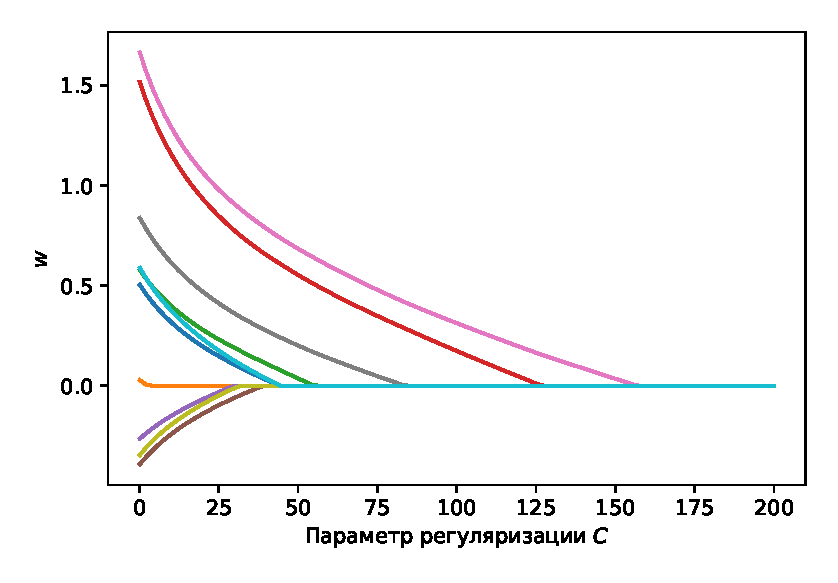
\includegraphics[width=0.5\textwidth]{../figures/log_reg_cs_exp.eps}
% 	\caption{Sample figure caption.}
% 	\label{fig:fig1}
% \end{figure}

% \subsection{Tables}
% See awesome Table~\ref{tab:table}.

% The documentation for \verb+booktabs+ (`Publication quality tables in LaTeX') is available from:
% \begin{center}
% 	\url{https://www.ctan.org/pkg/booktabs}
% \end{center}


% \begin{table}
% 	\caption{Sample table title}
% 	\centering
% 	\begin{tabular}{lll}
% 		\toprule
% 		\multicolumn{2}{c}{Part}                   \\
% 		\cmidrule(r){1-2}
% 		Name     & Description     & Size ($\mu$m) \\
% 		\midrule
% 		Dendrite & Input terminal  & $\sim$100     \\
% 		Axon     & Output terminal & $\sim$10      \\
% 		Soma     & Cell body       & up to $10^6$  \\
% 		\bottomrule
% 	\end{tabular}
% 	\label{tab:table}
% \end{table}

% \subsection{Lists}
% \begin{itemize}
% 	\item Lorem ipsum dolor sit amet
% 	\item consectetur adipiscing elit.
% 	\item Aliquam dignissim blandit est, in dictum tortor gravida eget. In ac rutrum magna.
% \end{itemize}


\bibliographystyle{unsrtnat}
\bibliography{references}

\end{document}